\documentclass[11pt]{article}

\input{../../preamble.tex}
% -----------------------------
% Packages
% -----------------------------
\usepackage[margin=1in]{geometry}
\usepackage{amsmath, amssymb, amsfonts}
\usepackage{mathtools}
\usepackage{graphicx}
\usepackage{float}
\usepackage{enumitem}
\usepackage{setspace}
\usepackage{hyperref}
\usepackage{fancyhdr}
\usepackage{titlesec}

\usepackage{subcaption} % in preamble
% -----------------------------
% Formatting
% -----------------------------
\onehalfspacing
\setlist[itemize]{noitemsep}
\setlist[enumerate]{noitemsep}

\pagestyle{fancy}
\fancyhf{}
\lhead{MECH 464 / EECE 442}
\rhead{Homework \#1}
\rfoot{\thepage}

\titleformat{\section}
  {\normalfont\Large\bfseries}{Exercise \thesection}{1em}{}

% -----------------------------
% Metadata
% -----------------------------
\title{Homework Assignment \#1}
\author{Dominic Klukas \\ 64348378}
\date{\today}

\begin{document}

\maketitle

% =============================
\section{}
% =============================
\textbf{(20 marks)}

Find on the web videos or images of:
\begin{itemize}
    \item CAT 215B excavator
    \item Kinova Gen 3 7-DOF robot
    \item ASIMO robot
\end{itemize}

Draw a schematic representation of \emph{one} of the following using the course joint
conventions (dimensions not required).

\textbf{Solution}.
We have here the requested images:
\begin{figure}[H]
    \centering
    \begin{subfigure}[t]{0.32\textwidth}
        \centering
        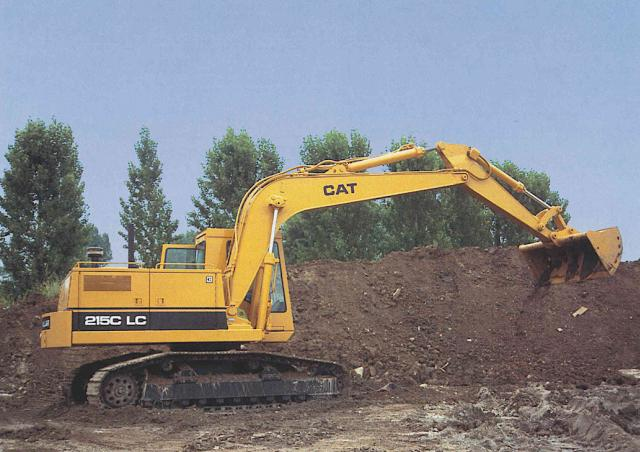
\includegraphics[height=4cm]{cat.jpg}
        \caption{CAT 215B Excavator}
        \label{fig:cat}
    \end{subfigure}\hfill
    \begin{subfigure}[t]{0.32\textwidth}
        \centering
        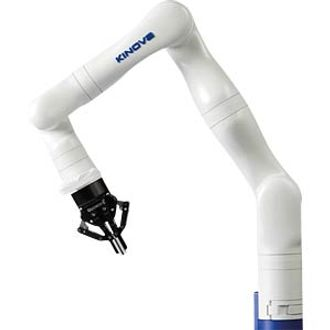
\includegraphics[height=4cm]{robot_arm.jpg}
        \caption{Kinova Gen 3 Arm}
        \label{fig:robotarm}
    \end{subfigure}\hfill
    \begin{subfigure}[t]{0.32\textwidth}
        \centering
        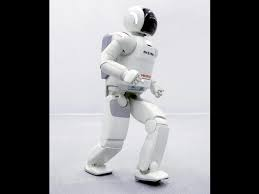
\includegraphics[height=4cm]{asimo.jpg}
        \caption{ASIMO Robot}
        \label{fig:asimo}
    \end{subfigure}
    \caption{Reference images for Exercise 1}
    \label{fig:exercise1_images}
\end{figure}

\begin{figure}[H]
    \centering
    % Put your final schematic image in the same folder as this .tex file
    % and replace the filename below.
    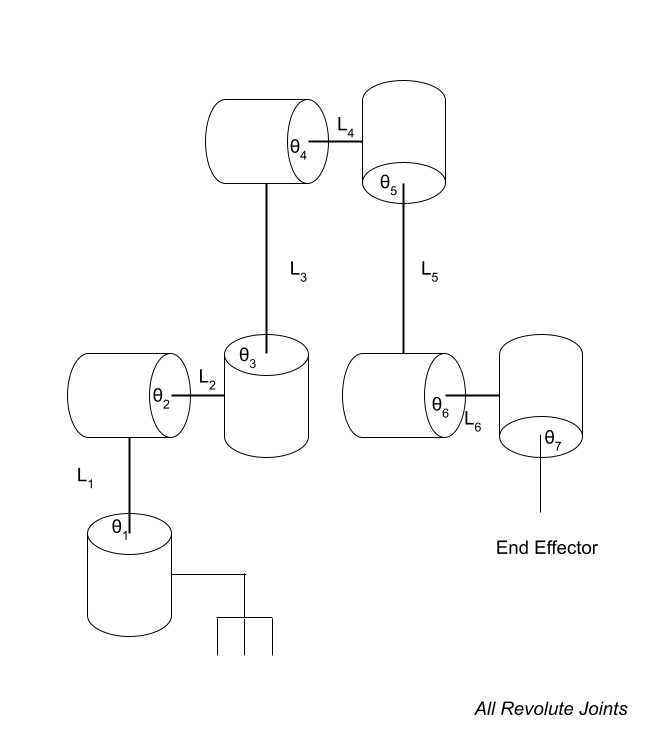
\includegraphics[width=0.5\textwidth]{Q1Schematic.png}
    \caption{Kinova Arm Schematic}
    \label{fig:kinova_schematic}
\end{figure}

% =============================
\section{}
% =============================
\textbf{(10 marks)}

Consider a three-link 3-DOF planar manipulator with $l_1 > l_2 > l_3$ and unconstrained
joint angles $\theta_1, \theta_2, \theta_3$.

In this problem, let $\tilde{o}$ be the point that $l_1$ is fixed onto and rotating about.
Now, since this is a planar manipulator, every reachable or dextrous point must be in the plane of operation, which I will call $P$.

For a point to be reachable, we require that $\tilde{x} = \tilde{o} + (\vec{l_1} + \vec{l_2} + \vec{l_3})$. Since joint angles are unconstrained, we have that this is the set $\{\tilde{x} \in P : |\tilde{x} - \tilde{o}| \leq l_1 + l_2 + l_3\}$.

For a point to be dextrous, we need the end effector to be able to reach the point from any angle.
Fix a point $\tilde{x}$.
Then, for any orientation $\theta_3$, we need $\tilde{o} + l_1 + l_2$ to be able to reach the point $\tilde{x} - \vec{l_3}$.
Mathematically, this means that the cirlce $\{\tilde{y} : |\tilde{y} - \tilde{x}| = l_3\}$ is contained in the points that can be reached by the end of link $l_2$, which is the circle $\{\tilde{x} \in P : |\tilde{x} - \tilde{o}| \leq l_1 + l_2 \}$.
Since $l_1 + l_2 > l_3$ (because $l_2 > l_3$), this is the case when $|\tilde{x} - \tilde{o}| \leq l_1 + l_2 - l_3$.
Therefore, the dextrous workspace is $\{\tilde{x} \in P : |\tilde{x} - \tilde{o} | \le l_1 + l_2 - l_3\}$.


% =============================
\section{}
% =============================
\textbf{(30 marks)}


Find a general procedure to compute the axis / angle representation of a rotation matrix
$Q$. Program it in MATLAB and verify it for the examples provided. Clearly describe your algorithm and hand in your MATLAB code as well as working examples.

\textbf{Solution.}
\subsection*{Algorithm Description}
First, compute the eigenvalues of $Q$.
Since $Q$ is a rotation matrix, there are 3: $e^{\pm i\theta}, 1$.
In particular, if $\theta > 180$, the rotation matrix will be indistinguishable from a rotation matrix with axis $\vec{s} \to -\vec{s}$ and $\theta < 180$, so choose the only eigenvalue with a positive imaginary component, and compute $\theta = \arctan(\textrm{Im}(v_1) / \textrm{Re}(v_1))$.

The axis will be the eigenvector of the eigenvalue $1$, so compute it.
However, we still need to determine the sense of the axis, so that the vector describing the axis obeys the right hand rule.
To do so, we take any vector $x$ that isn't parallel to the axis and rotate it, and then take the cross product with $Q x$.
With this cross product, we take the dot product with the axis vector.
If this dot product is positive, the sense is already correct.
If not, we flip the axis vector.
To choose which vector to do, we try the standard co-ordinate axes and choose the one with the smallest dot product with the axis vector.

\subsection*{Worked Example}

Let's work the example for rotation matrix 1.
We seek to find the axis-angle for the matrix:
\[
    Q = \begin{pmatrix} 0.6152 & -0.4103 & 0.6732\\ 0.6983 & 0.6800 & -0.2237\\ -0.3660 & 0.6077 & 0.7048 \end{pmatrix} 
.\] 
Computing the eigenvectors/eigenvalues for 3x3 matrices is tedious and not particularly illuminating, so I will simply report the result of matlab's computation:
\[
\lambda = 1, \frac{1}{2} \pm \sqrt{3}/2 i
.\] 
Then, we have:
\[
\theta = \arctan\left(\frac{\sqrt{3} / 2}{2}\right) = 60^{\circ}
.\] 

The eigenvector corresponding to eigenvalue $1$ is $[0.48, 0.6, 0.64]^{\top}$.
The unit vector $\hat{i}, \hat{j}, \hat{k}$ with the smallest dot product with this vector is $\hat{i}$, with a value of $0.48$.
We compute:
\[
Q\cdot [1, 0, 0]^{\top} = [0.6152, 0.6983, -0.3660]^{\top}
.\] 
Next,
\[
[1, 0, 0]^{\top} \times Q \cdot [1, 0, 0]^{\top} = [0, 0.3660, 0.6983]^{\top}
.\] 
Clearly, $[0.48, 0.6, 0.64] \cdot [0, 0.3660, 0.6983]^{\top} > 0
$, so we have that the sense of our axis is correct.

Therefore,
\begin{align*}
    \theta &= 1.0472 \text{ rad}, 60 \text{ degrees}\\
    \text{axis} &= [0.48, 0.6, 0.64]
.\end{align*}

\subsection*{Code}

\begin{verbatim}
% MATLAB implementation
function [axis, angle] = axisAngleFromRotation(Q)
    tol = 1e-3;
    [V, D] = eig(Q);
    eigenvalues = diag(D);
    idx = find(imag(eigenvalues) > 0, 1);
    if ~isempty(idx)
        theta = atan2(imag(eigenvalues(idx)), real(eigenvalues(idx)));
    else
        if any(abs(eigenvalues+1) < 0 + tol)
            theta = pi;
        else
            theta = 0;
        end
    end
    
    axis_idx = find(abs(eigenvalues - 1) < tol, 1);
    axis = V(:, axis_idx);
    
    e1 = [1;0;0];
    e2 = [0;1;0];
    e3 = [0;0;1];
    E = eye(3);
    
    [~, y_index] = min(abs([dot(axis, e1), dot(axis, e2), dot(axis, e3)]));
    y = E(:,y_index);
    y_rot = Q*y;
    sense_test = dot(cross(y, y_rot), axis);
    
    if sense_test < -tol
        axis = -axis;
    end
    axis = axis / norm(axis);
    angle = theta;
end
\end{verbatim}

\subsection*{Verification}

We have here the required verification examples:

\begin{verbatim}
Q1:
  axis  = [0.479979 0.599983 0.640031]^T
  angle = 1.047208849083 rad (60.000647 deg)

Q2:
  axis  = [0.360019 0.799977 0.480023]^T
  angle = 1.047196849304 rad (59.999960 deg)

Q3:
  axis  = [0.480002 0.600052 0.639950]^T
  angle = 0.523590593707 rad (29.999531 deg)

Q4:
  axis  = [0.800000 0.360000 0.480000]^T
  angle = 1.570796326795 rad (90.000000 deg)

Q5:
  axis  = [0.577350 0.577350 0.577350]^T
  angle = 0.785440409113 rad (45.002421 deg)

I:
  axis  = [1.000000 0.000000 0.000000]^T
  angle = 0.000000000000 rad (0.000000 deg)
\end{verbatim}

% =============================
\end{document}

